\documentclass[12pt]{article}
\usepackage[a4paper,margin=1in]{geometry}
\usepackage{graphicx}
\usepackage{amsmath}
\usepackage{hyperref}
\usepackage{minted}

\begin{document}

%-------------------- Title Page --------------------
\title{Laboratory 1: Circuit Designs and Testing}
\author{Shein Htike \and Brandon Vasquez}
\date{CSC 343 Spring 2025}
\maketitle

\tableofcontents
\clearpage

\section{Exercise A: 8x1 Multiplexer Using Logic Gates}
\subsection{Objective}
The goal of this exercise is to create an 8x1 multiplexer in two ways: using logic gates and using VHDL code.
\subsection{Functionality and Specifications}
\subsubsection{Logic}
The output of the 8×1 multiplexer is given by the following logic equation:

\begin{equation}
\begin{split}
\text{output} =\,& \overline{S_2}\,\overline{S_1}\,\overline{S_0}\,I_0 \ \vee\ \overline{S_2}\,\overline{S_1}\,S_0\,I_1 \ \vee \\[1mm]
                & \overline{S_2}\,S_1\,\overline{S_0}\,I_2 \ \vee\ \overline{S_2}\,S_1\,S_0\,I_3 \ \vee \\[1mm]
                & S_2\,\overline{S_1}\,\overline{S_0}\,I_4 \ \vee\ S_2\,\overline{S_1}\,S_0\,I_5 \ \vee \\[1mm]
                & S_2\,S_1\,\overline{S_0}\,I_6 \ \vee\ S_2\,S_1\,S_0\,I_7 
\end{split}
\end{equation}

In this multiplexer design, we select one of the eight inputs, $I_{0}$ through $I_{7}$ and connect it to a single output based on the binary value of the three select signals, $S_{2}$, $S_{1}$, and $S_{0}$ (with $S_{2}$ being the most significant bit).
\clearpage
\subsubsection{Circut Design}
In order to implement the 8x1 multiplexer, we created this circuit design in Intel Quartus Prime.
This circuit was then compiled into VHDL and imported into ModelSim in order to simulate and test our design. \\
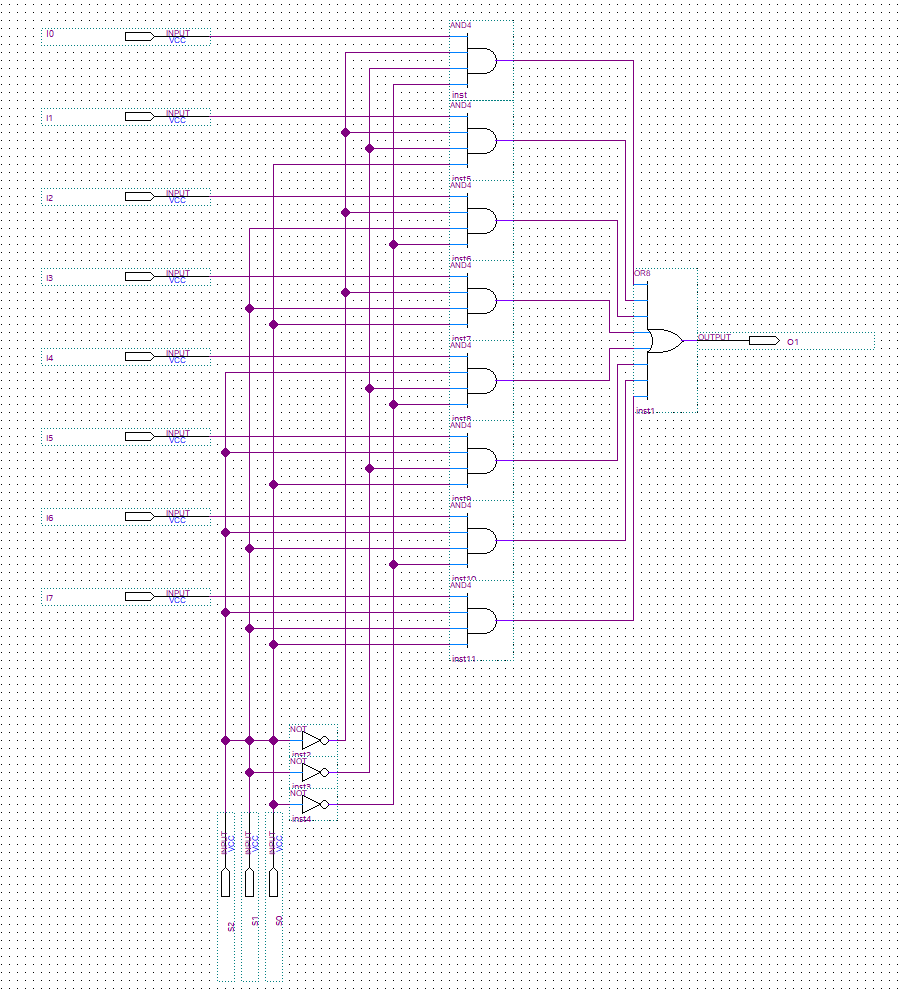
\includegraphics[width=\textwidth]{8x1multiplexer.png}
\clearpage
\subsubsection{VHDL Code}
I also redesigned this multiplexer in VHDL using behavioral modeling.
\begin{minted}{vhdl}
    library IEEE;
    use IEEE.std_logic_1164.all;
    
    entity multiplexer8x1v2 is
        port (
            I : in  std_logic_vector(7 downto 0);
            S : in  std_logic_vector(2 downto 0);
            O : out std_logic
        );
    end multiplexer8x1v2;
    
    architecture Behavioral of multiplexer8x1v2 is
    begin
        with S select
            O <= I(0) when "000",
                 I(1) when "001",
                 I(2) when "010",
                 I(3) when "011",
                 I(4) when "100",
                 I(5) when "101",
                 I(6) when "110",
                 I(7) when "111",
                 '0'    when others;  -- Default case if needed
    end Behavioral;
\end{minted}
\clearpage

\subsection{Simulation}
I wrote VHDL to simulate both versions of the circuit.
\subsubsection{Structural Model Test Bench}

\begin{minted}{vhdl}
LIBRARY IEEE;
USE IEEE.STD_LOGIC_1164.ALL;
USE IEEE.STD_LOGIC_TEXTIO.ALL;
USE std.textio.ALL;

ENTITY tb_multiplexer8x1 IS
END tb_multiplexer8x1;

ARCHITECTURE test OF tb_multiplexer8x1 IS
    SIGNAL I0 : STD_LOGIC := '0';
    SIGNAL I1 : STD_LOGIC := '0';
    SIGNAL I2 : STD_LOGIC := '0';
    SIGNAL I3 : STD_LOGIC := '0';
    SIGNAL I4 : STD_LOGIC := '0';
    SIGNAL I5 : STD_LOGIC := '0';
    SIGNAL I6 : STD_LOGIC := '0';
    SIGNAL I7 : STD_LOGIC := '0';
    SIGNAL S2 : STD_LOGIC := '0';
    SIGNAL S1 : STD_LOGIC := '0';
    SIGNAL S0 : STD_LOGIC := '0';
    SIGNAL O1 : STD_LOGIC;

    COMPONENT mux8to1_structural IS
        PORT (
            I0 : IN STD_LOGIC;
            I2 : IN STD_LOGIC;
            I3 : IN STD_LOGIC;
            I1 : IN STD_LOGIC;
            I4 : IN STD_LOGIC;
            I5 : IN STD_LOGIC;
            I6 : IN STD_LOGIC;
            I7 : IN STD_LOGIC;
            S2 : IN STD_LOGIC;
            S1 : IN STD_LOGIC;
            S0 : IN STD_LOGIC;
            O1 : OUT STD_LOGIC
        );
    END COMPONENT;

BEGIN
    uut : mux8to1_structural
    PORT MAP(I0, I2, I3, I1, I4, I5, I6, I7, S2, S1, S0, O1);

    PROCESS
    BEGIN
        S2 <= '0';
        S1 <= '0';
        S0 <= '0';
        WAIT FOR 10 ns;
        I0 <= '1';
        WAIT FOR 10 ns;
        I0 <= '0';

        S2 <= '0';
        S1 <= '0';
        S0 <= '1';
        WAIT FOR 10 ns;
        I1 <= '1';
        WAIT FOR 10 ns;
        I1 <= '0';

        S2 <= '0';
        S1 <= '1';
        S0 <= '0';
        WAIT FOR 10 ns;
        I2 <= '1';
        WAIT FOR 10 ns;
        I2 <= '0';

        S2 <= '0';
        S1 <= '1';
        S0 <= '1';
        WAIT FOR 10 ns;
        I3 <= '1';
        WAIT FOR 10 ns;
        I3 <= '0';

        S2 <= '1';
        S1 <= '0';
        S0 <= '0';
        WAIT FOR 10 ns;
        I4 <= '1';
        WAIT FOR 10 ns;
        I4 <= '0';

        S2 <= '1';
        S1 <= '0';
        S0 <= '1';
        WAIT FOR 10 ns;
        I5 <= '1';
        WAIT FOR 10 ns;
        I5 <= '0';

        S2 <= '1';
        S1 <= '1';
        S0 <= '0';
        WAIT FOR 10 ns;
        I6 <= '1';
        WAIT FOR 10 ns;
        I6 <= '0';

        S2 <= '1';
        S1 <= '1';
        S0 <= '1';
        WAIT FOR 10 ns;
        I7 <= '1';
        WAIT FOR 10 ns;
        I7 <= '0';
    END PROCESS;
END test;

\end{minted}
This code selects inputs 0 through 7 and toggles them while they are selected to show that the output corresponds to the selected input.

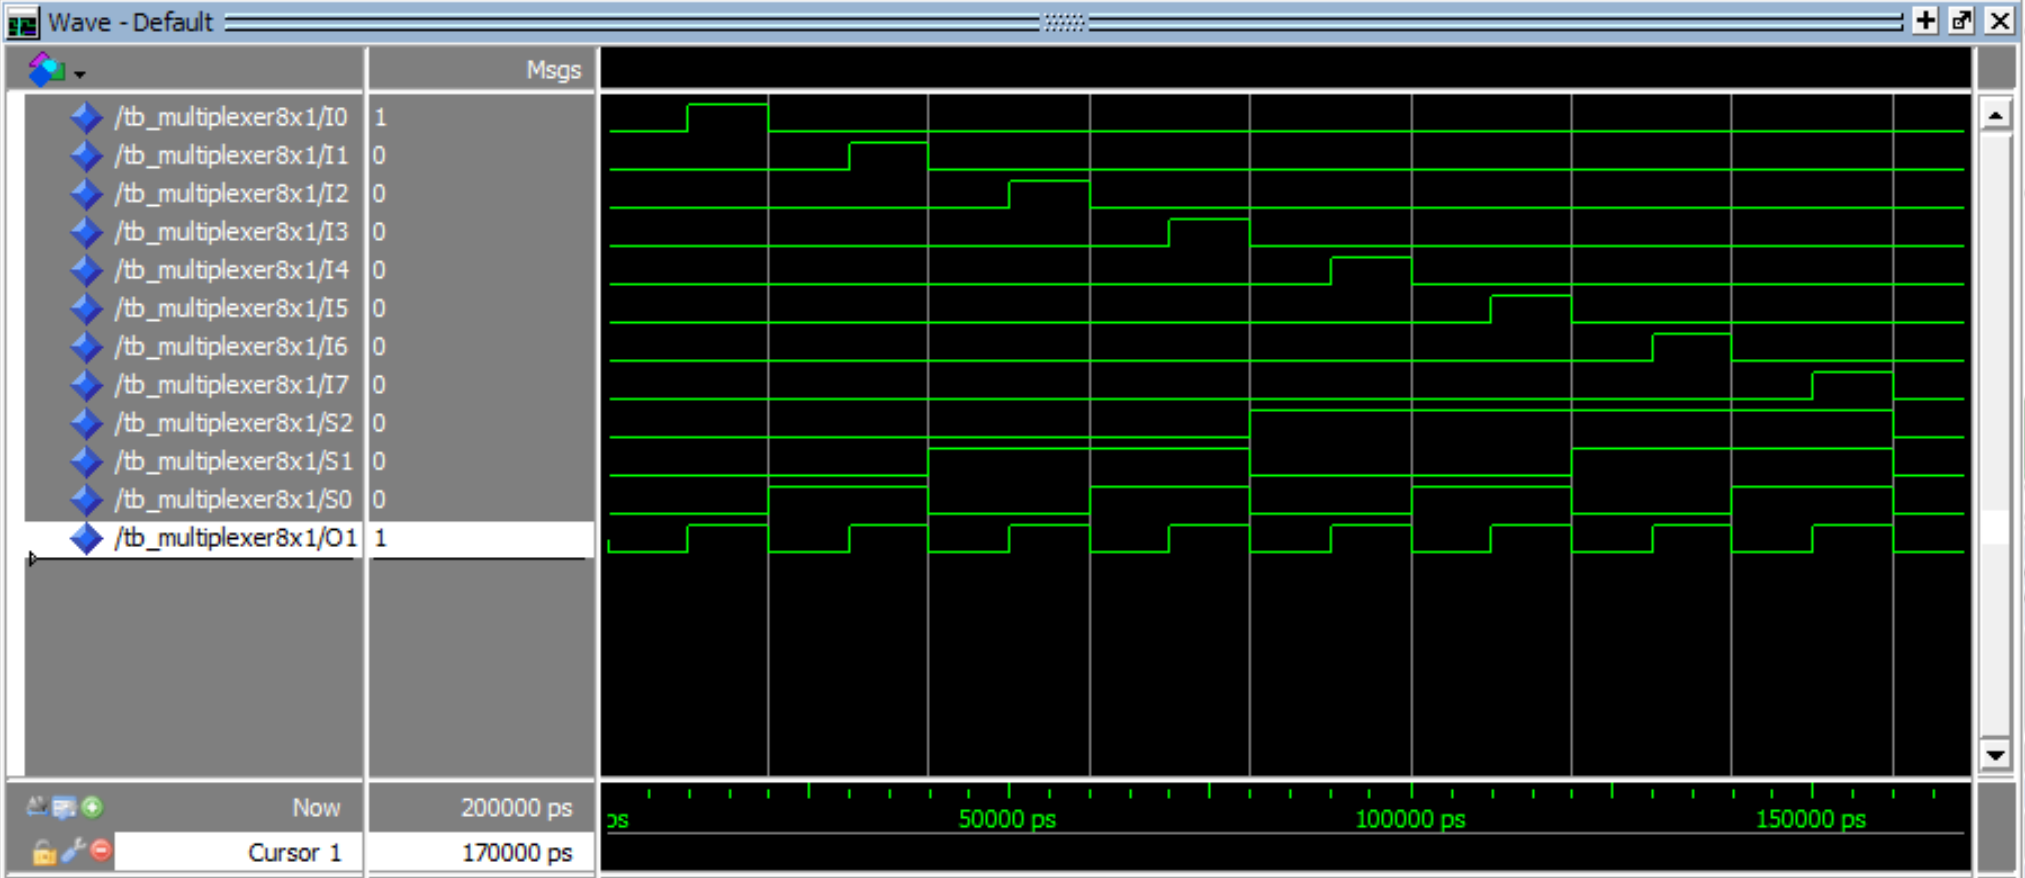
\includegraphics[width=\textwidth]{mux_structural.png}
\clearpage
\subsubsection{Behavioral Model Test Bench}
I also wrote test bench code for the behavioral model multiplexer. This code was essentially the same as the previous test bench for the structural model. The only difference is that the inputs and the select signals were vectors.
\begin{minted}{vhdl}
    LIBRARY IEEE;
USE IEEE.STD_LOGIC_1164.ALL;
USE IEEE.STD_LOGIC_TEXTIO.ALL;
USE STD.TEXTIO.ALL;

ENTITY tb_multiplexer8x1v2 IS
END tb_multiplexer8x1v2;

ARCHITECTURE test OF tb_multiplexer8x1v2 IS
    SIGNAL I : STD_LOGIC_VECTOR(7 DOWNTO 0) := (OTHERS => '0');
    SIGNAL S : STD_LOGIC_VECTOR(2 DOWNTO 0) := "000";
    SIGNAL O : STD_LOGIC;
    COMPONENT multiplexer8x1v2 IS
        PORT (
            I : IN  STD_LOGIC_VECTOR(7 DOWNTO 0);
            S : IN  STD_LOGIC_VECTOR(2 DOWNTO 0);
            O : OUT STD_LOGIC
        );
    END COMPONENT;
BEGIN
    uut : multiplexer8x1v2
        PORT MAP (
            I => I,
            S => S,
            O => O
        );
    PROCESS
    BEGIN
        S <= "000";
        I <= (OTHERS => '0');
        WAIT FOR 10 ns;
        I(0) <= '1';
        WAIT FOR 10 ns;
        I(0) <= '0';
        S <= "001";
        I <= (OTHERS => '0');
        WAIT FOR 10 ns;
        I(1) <= '1';
        WAIT FOR 10 ns;
        I(1) <= '0';
        S <= "010";
        I <= (OTHERS => '0');
        WAIT FOR 10 ns;
        I(2) <= '1';
        WAIT FOR 10 ns;
        I(2) <= '0';
        S <= "011";
        I <= (OTHERS => '0');
        WAIT FOR 10 ns;
        I(3) <= '1';
        WAIT FOR 10 ns;
        I(3) <= '0';
        S <= "100";
        I <= (OTHERS => '0');
        WAIT FOR 10 ns;
        I(4) <= '1';
        WAIT FOR 10 ns;
        I(4) <= '0';
        S <= "101";
        I <= (OTHERS => '0');
        WAIT FOR 10 ns;
        I(5) <= '1';
        WAIT FOR 10 ns;
        I(5) <= '0';
        S <= "110";
        I <= (OTHERS => '0');
        WAIT FOR 10 ns;
        I(6) <= '1';
        WAIT FOR 10 ns;
        I(6) <= '0';
        S <= "111";
        I <= (OTHERS => '0');
        WAIT FOR 10 ns;
        I(7) <= '1';
        WAIT FOR 10 ns;
        I(7) <= '0';
        WAIT;
    END PROCESS;
END test;
\end{minted}
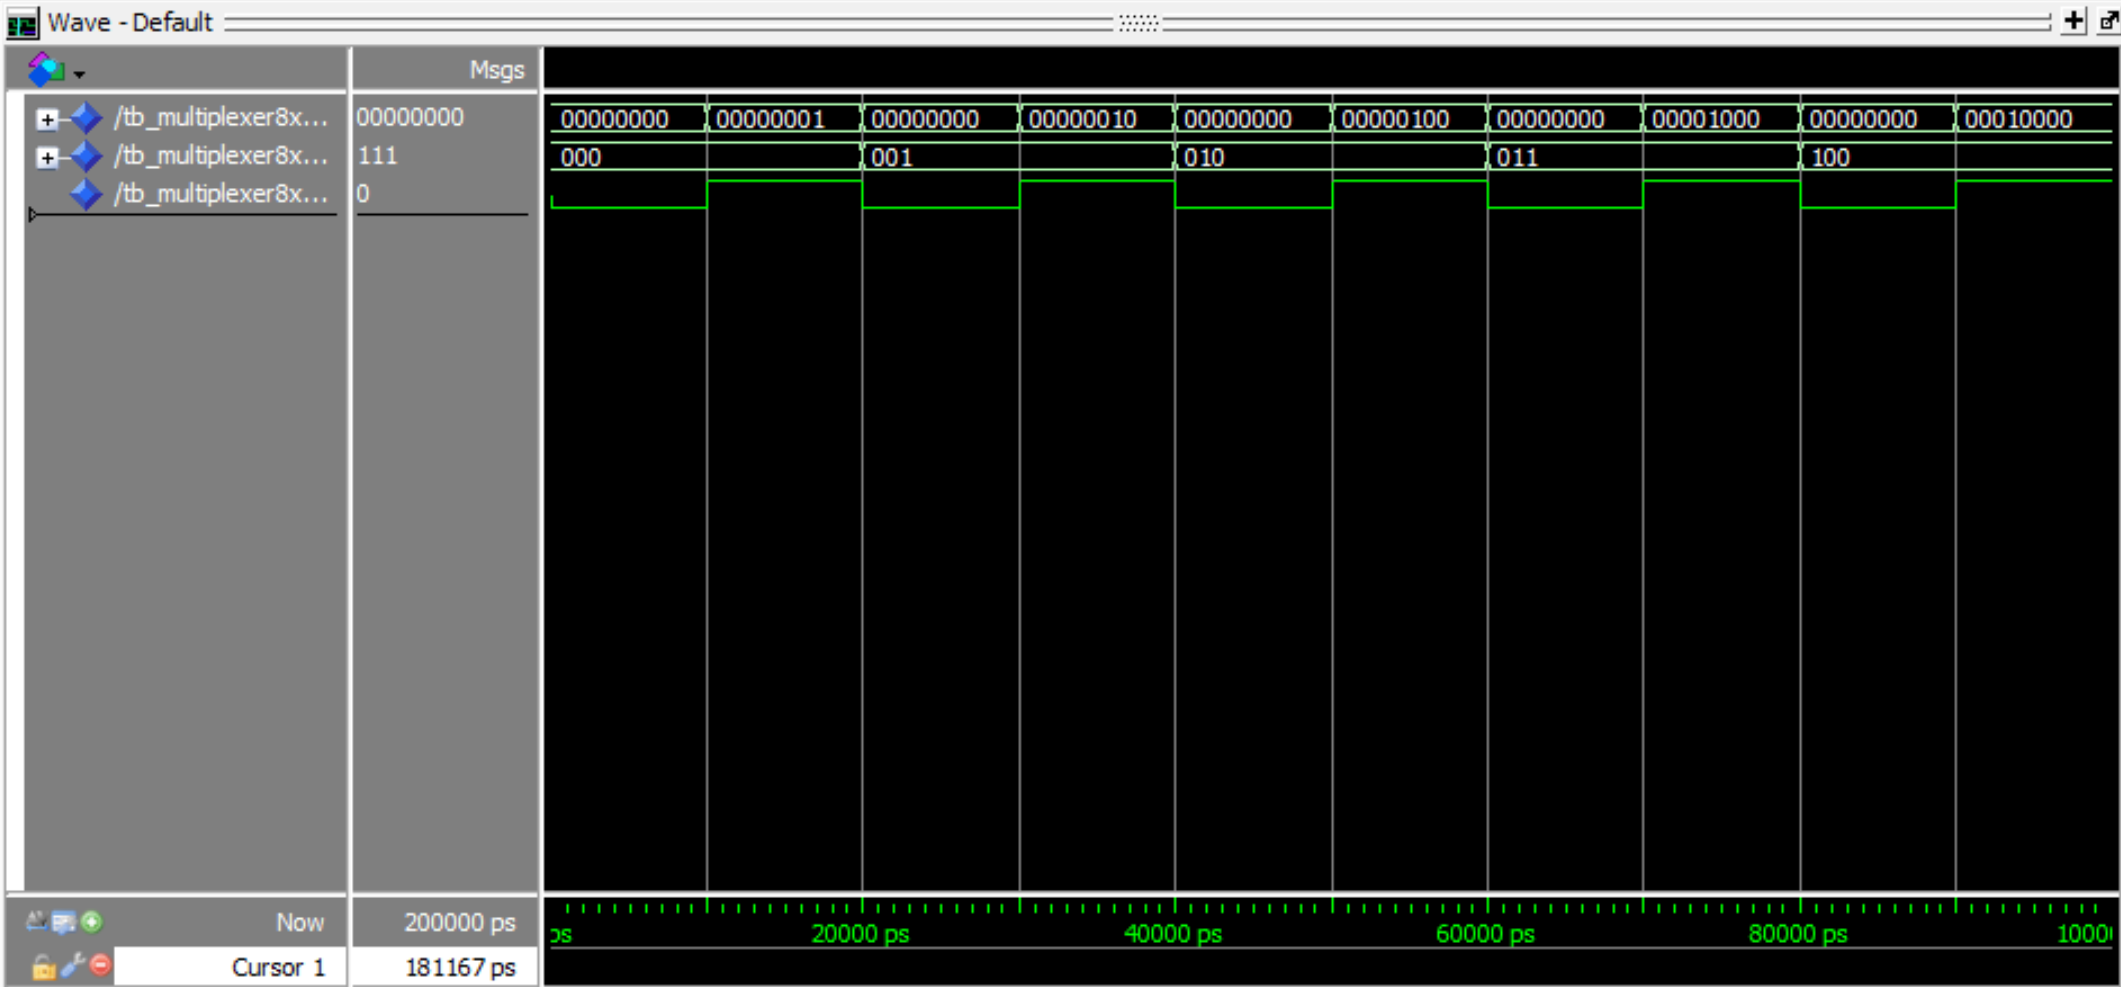
\includegraphics[width=\textwidth]{mux_behavioral.png}
\clearpage
\section{Exercise B: 1x8 De-Multiplexer Using 1x4 and 1x2 De-Multiplexers}
\subsection{Objective}

\subsection{Functionality and Specifications}

\subsection{Simulation}

\clearpage
\section{Exercise C: 3-to-8 Decoder}
\subsection{Objective}

\subsection{Functionality and Specifications}

\subsection{Simulation}

\clearpage
\section{Exercise D: 8-to-3 Priority Encoder}
\subsection{Objective}

\subsection{Functionality and Specifications}
\[
\begin{aligned}
Y_2 &= D_7 + D_6 + D_5 + D_4,\\[1mm]
Y_1 &= D_7 + D_6 + \overline{D_7 + D_6}\,(D_3 + D_2),\\[1mm]
Y_0 &= D_7 + \overline{D_7 + D_6}\,D_5 + \overline{D_7 + D_6 + D_5}\,D_3 + \overline{D_7 + D_6 + D_5 + D_4}\,D_1.
\end{aligned}
\]

\subsection{Simulation}

\clearpage
\section{Exercise E: Set-Reset Flip-Flop \& D Flip-Flop (Positive Edge Trigger)}
\subsection{Objective}

\subsection{Functionality and Specifications}

\subsection{Simulation}

\section{Conclusions}

\end{document}